A cut and count analysis is performed using the asymptotic \CLs modified frequentist approach to place upper limits on the signal hypotheses~\cite{Junk:1999kv,Read:411537:Lyons}. Systematic uncertainties are integrated over with a log-normal probability function, while statistical uncertainties are modeled by $\Gamma$ distributions whose widths are taken to be the number of simulated events in MC samples.

Figure~\ref{fig:limit_plots} shows the asymptotic upper limits on $\sigma(\HepProcess{\Pp\Pp \to \LQ\LQbar})$ as a function of leptoquark mass in 2016, 2017, and 2018 datasets, together with the NLO prediction of scalar leptoquark pair production cross sections. The theoretical cross section curves are represented for the renormalization and factorization scale $\mu$, varied by up by $2\MLQ$ and down by $\MLQ/2$. PDF uncertainties are accounted for in the theory cross sections. 

Asymptotic upper limits on the combination of 2016, 2017, and 2018 datasets, shown in Figure~\ref{fig:limit_plot_combined} with the theory prediction, exclude leptoquark masses below \SI{1803}{\GeV}. This is an improvement of \SI{273}{\GeV} over the previous results with 2016 data~\cite{CMSLQ2_2016}.

\begin{figure}[H]
  \centering
  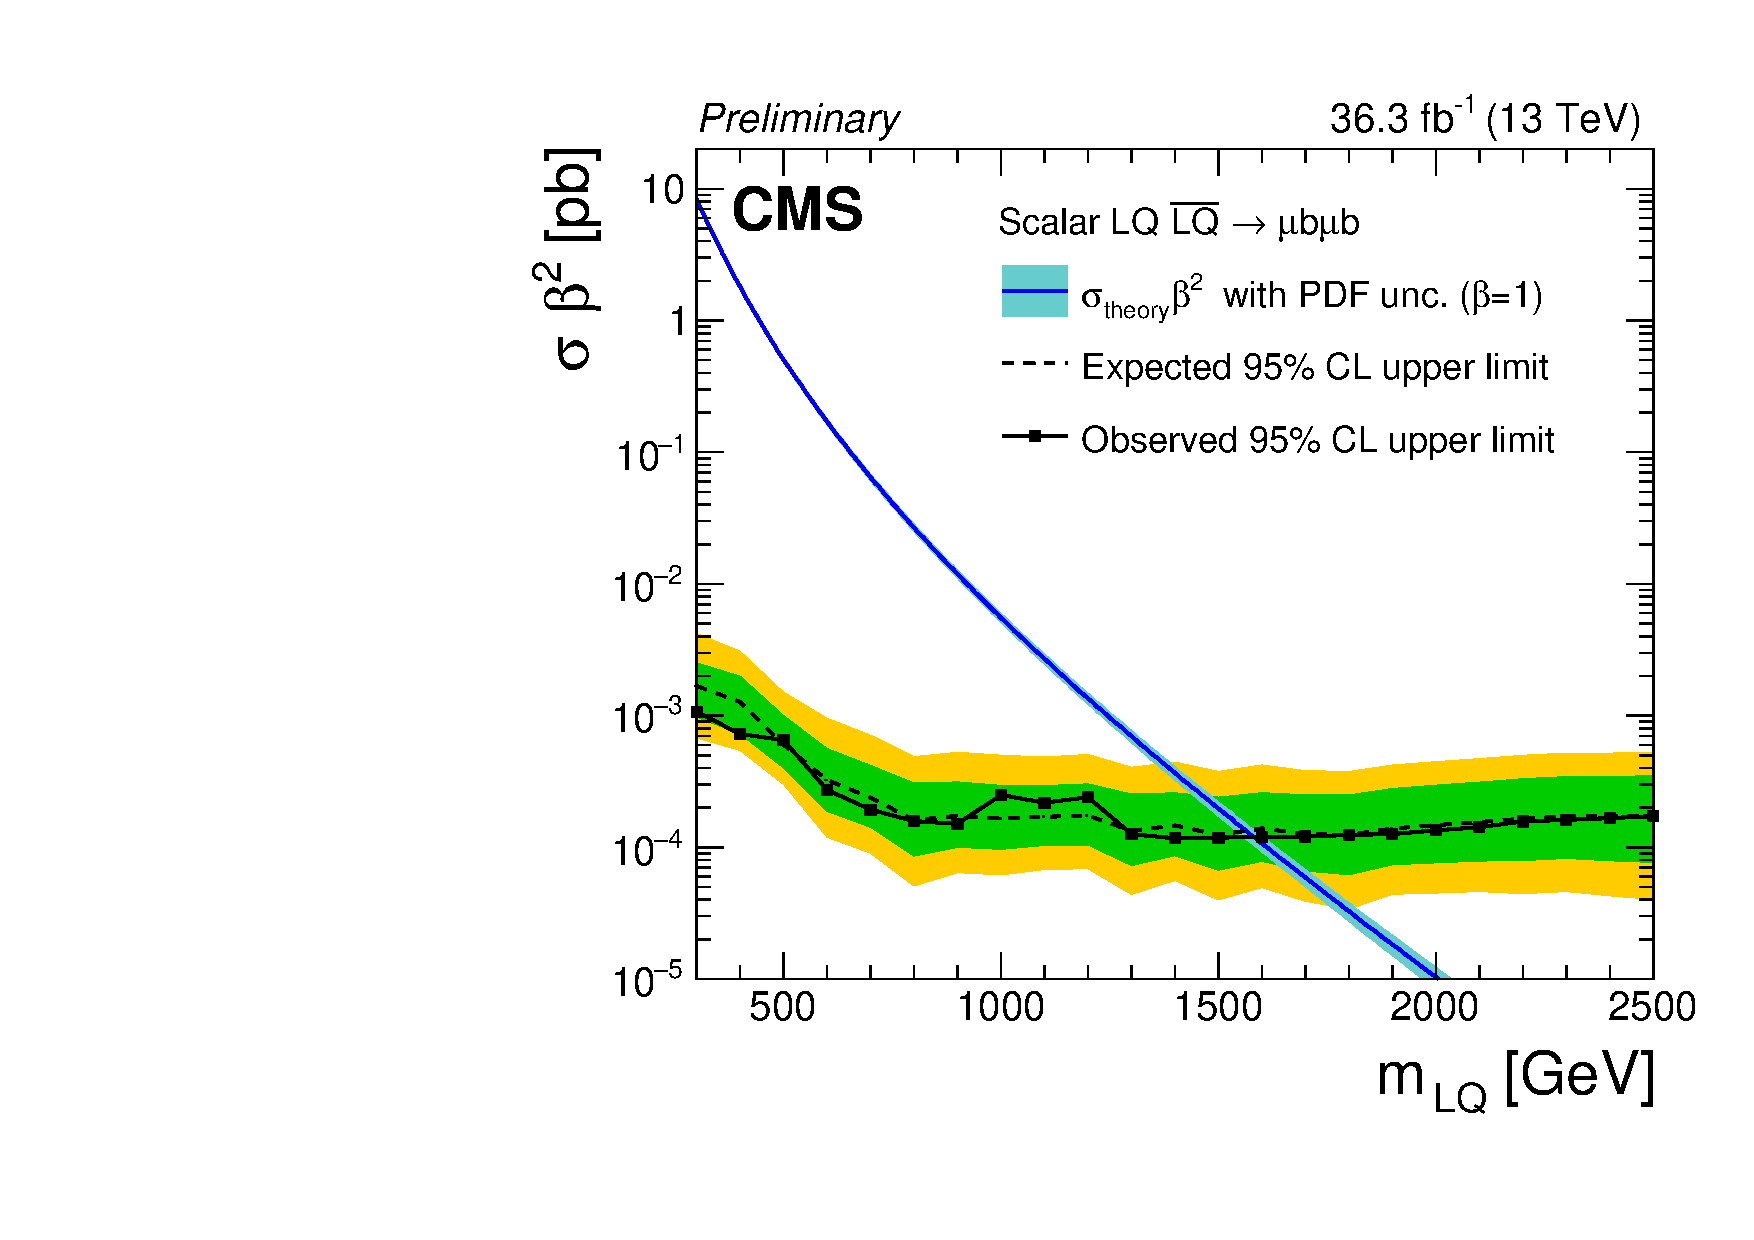
\includegraphics[width=0.32\textwidth]{Images/Analysis/Limits/BR_Sigma_MuMu_2016.pdf}
  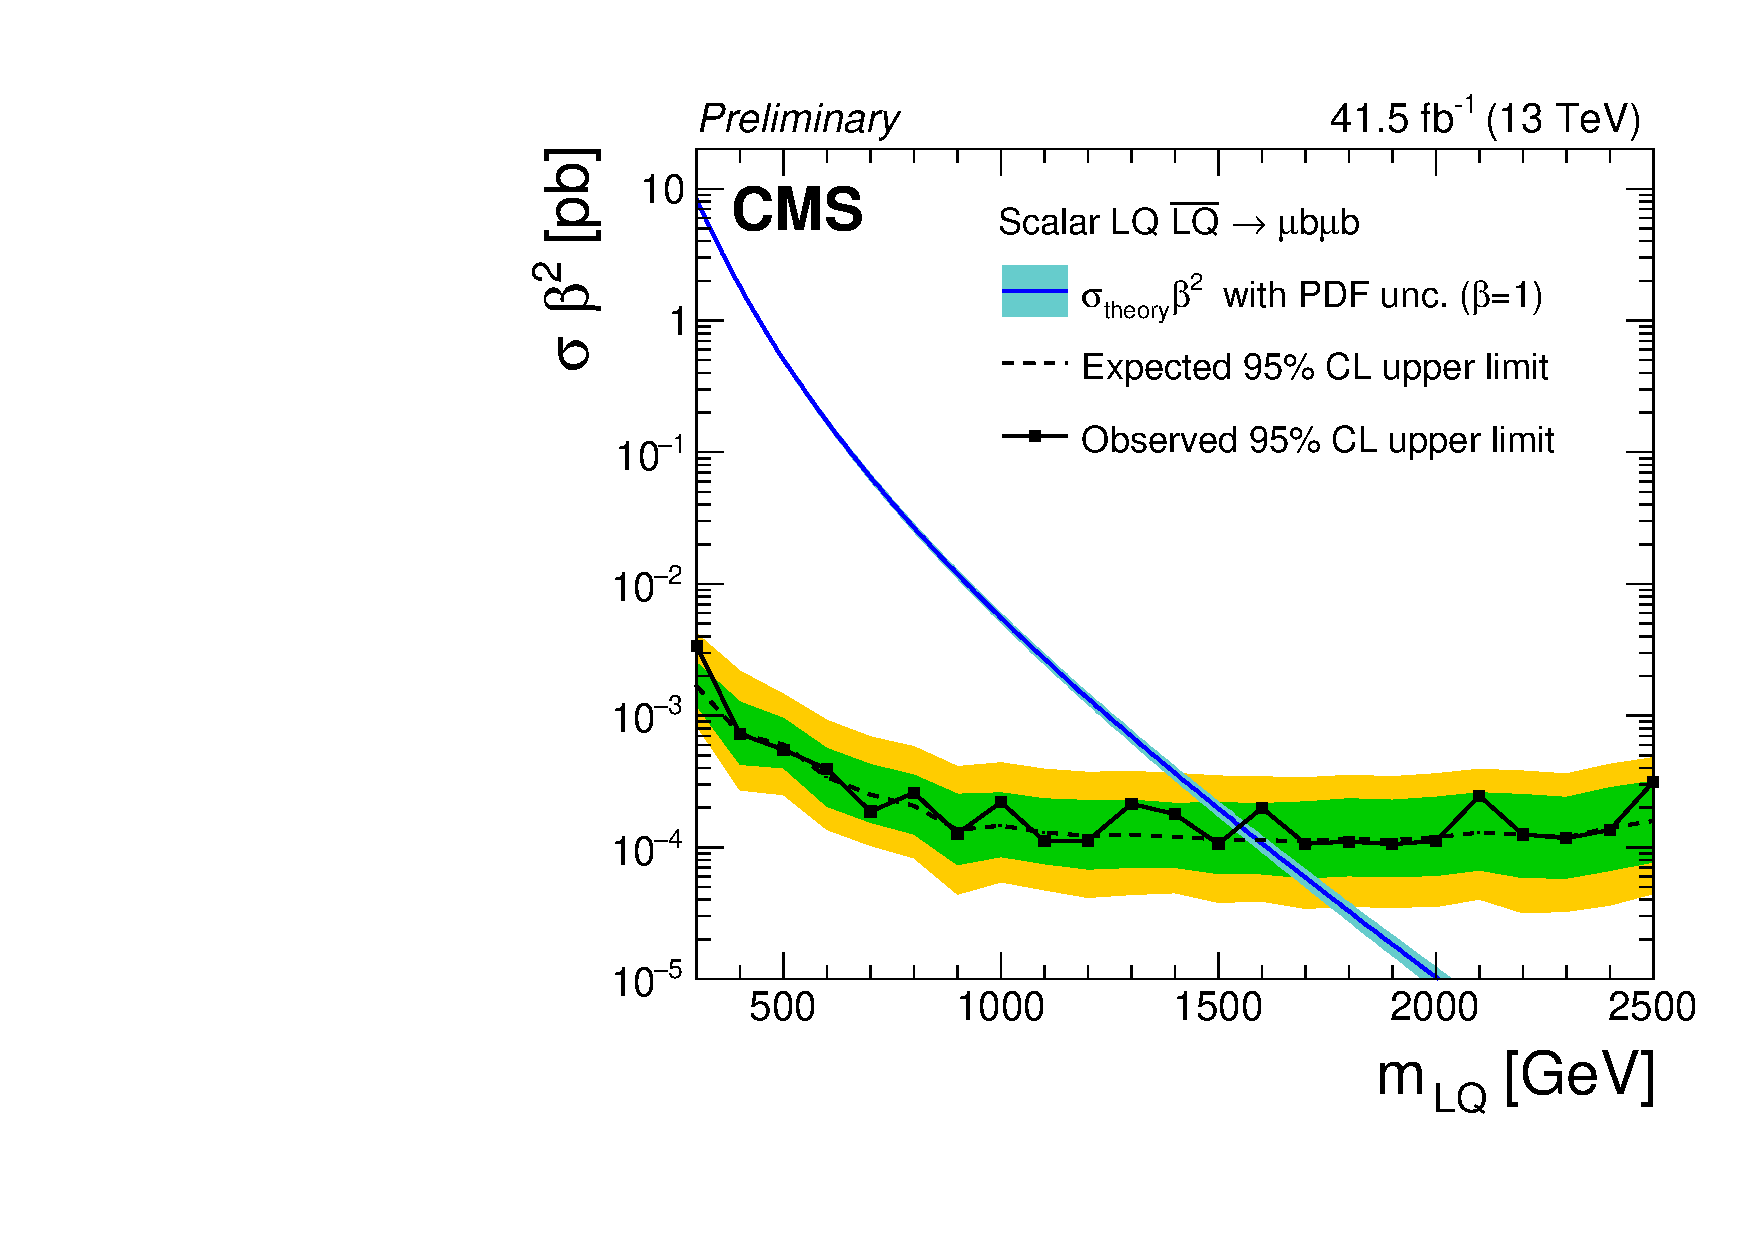
\includegraphics[width=0.32\textwidth]{Images/Analysis/Limits/BR_Sigma_MuMu_2017.pdf}
  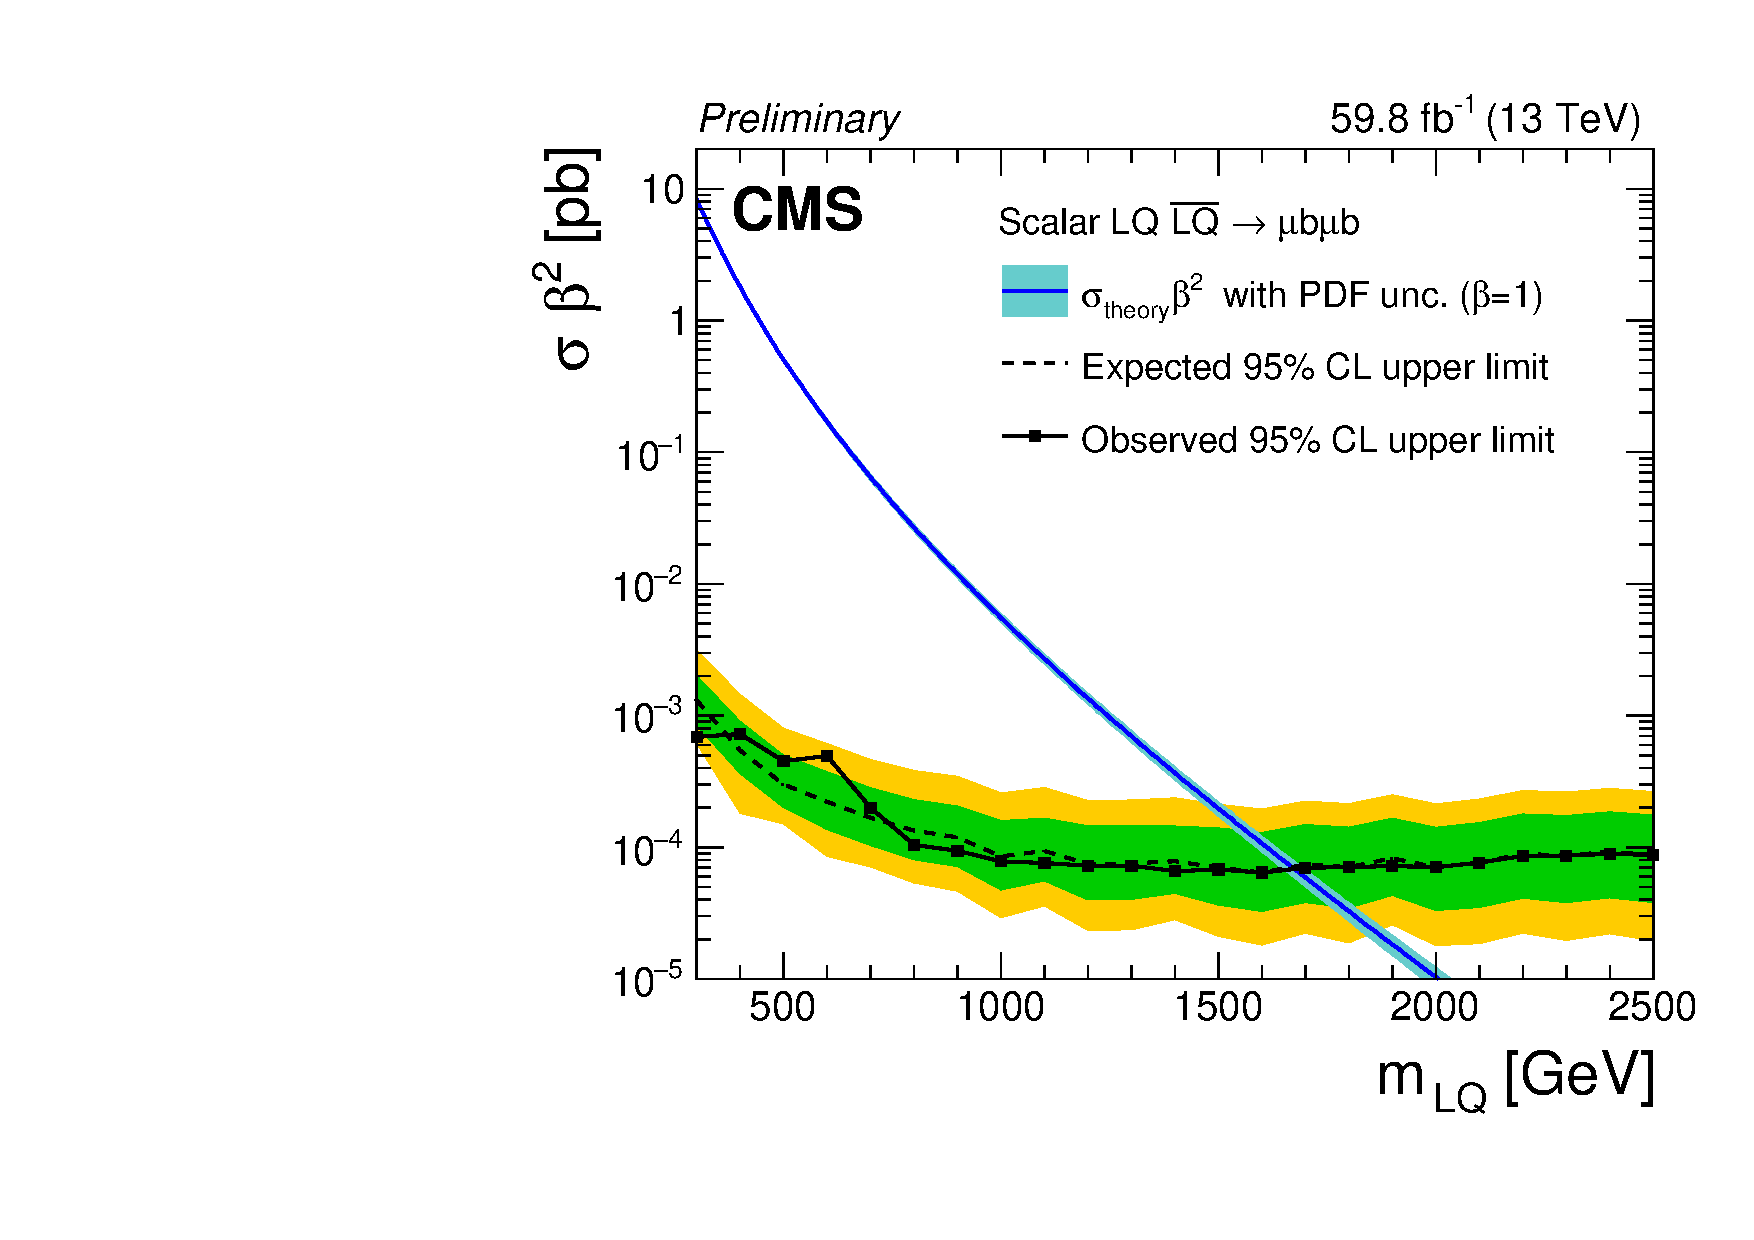
\includegraphics[width=0.32\textwidth]{Images/Analysis/Limits/BR_Sigma_MuMu_2018.pdf}
  \caption{The asymptotic upper limits at \SI{95}{\%} \CL on the leptoquark pair production cross section times squared branching fraction as a function of leptoquark mass obtained with the \mumubj analysis with 2016 (left), 2017 (middle), and 2018 (right) datasets. The expected limits and uncertainty bands represent the median expected limits and the \SI{68}{\%} and \SI{95}{\%} confidence intervals. The \xsecTheory curves and their bands represent, respectively, the theoretical scalar leptoquark pair production cross section and the uncertainties due to the choice of PDF and renormalization/factorization scales.}
  \label{fig:limit_plots}
\end{figure}

\begin{figure}[H]
  \centering
  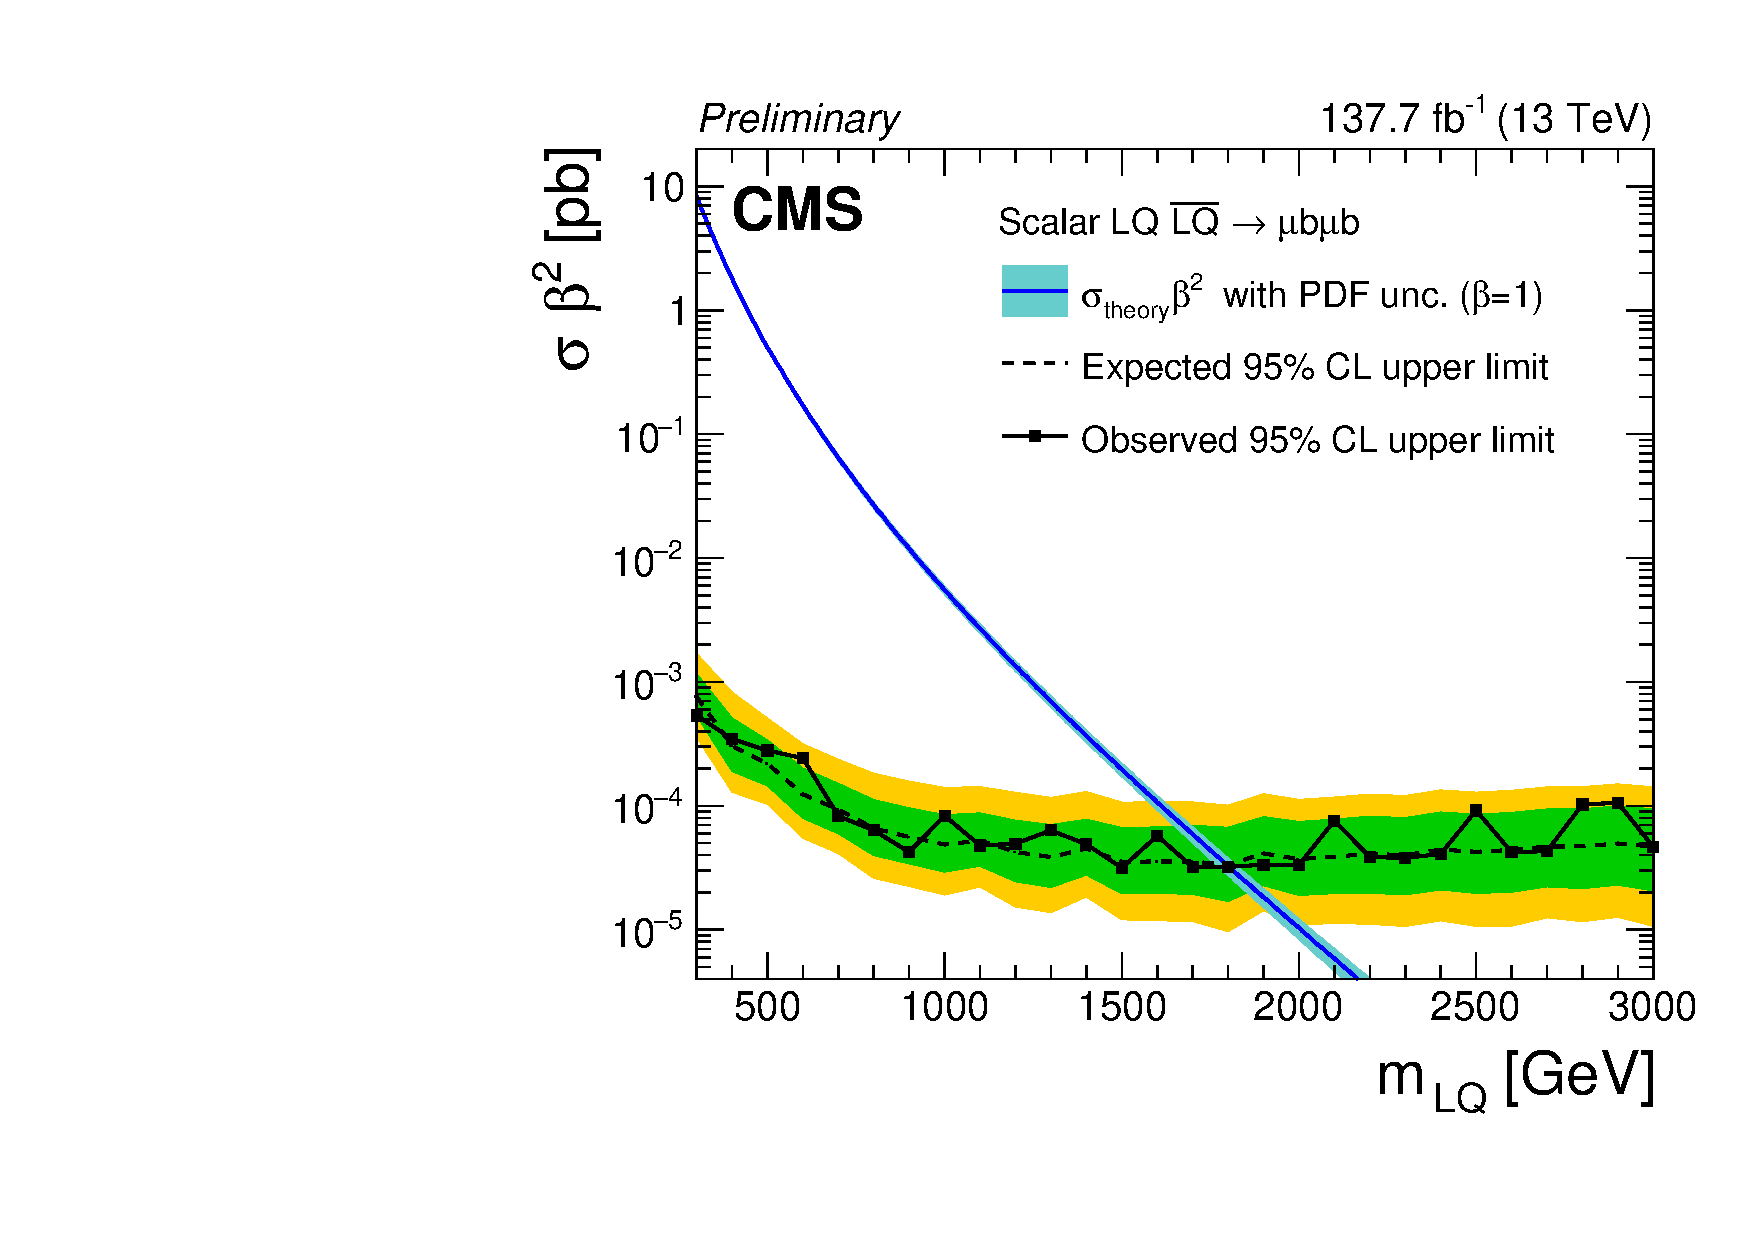
\includegraphics[width=\textwidth]{Images/Analysis/Limits/BR_Sigma_MuMu_Combined.pdf}
  \caption{The asymptotic upper limits at \num{95}{\%} \CL on the leptoquark pair production cross section $\sigma$ times squared branching fraction $\beta^2$ as a function of leptoquark mass obtained with the \mumubj analysis. The expected limits and uncertainty bands represent the median expected limits and the \SI{68}{\%} and \SI{95}{\%} confidence intervals. The \xsecTheory curves and their bands represent, respectively, the theoretical scalar leptoquark pair production cross section and the uncertainties due to the choice of PDF and renormalization/factorization scales.}
  \label{fig:limit_plot_combined}
\end{figure}